%!TEX root = ../../../main.tex



	\subsection{Sideband} \label{subsubsec::sideband}

		\begin{figure}[tp]
			\centering
			\testbox{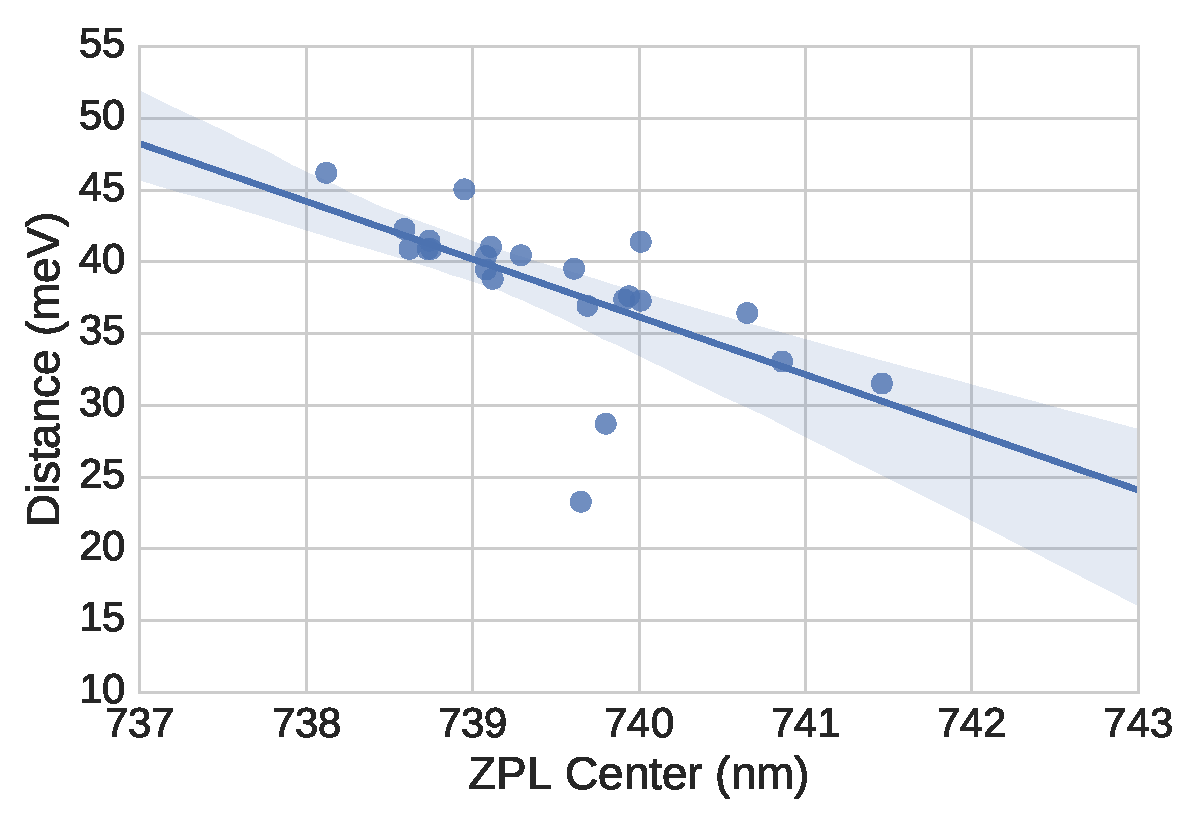
\includegraphics[trim = 0 0 0 0,  clip= true, width = 0.49\textwidth]{./pics/sideband_regression.pdf}}
			\caption{Shift of dominant sideband peak from the \ZPL in spectra of \sivs (\vl, samples \insituF, \insituS, \insituH) vs. ZPL \cwl. The linear fit shows that the shift decreases with increasing ZPL center wavelength. The shaded area is the 95\% confidence interval.}
			\label{fig::sideband_fit}
		\end{figure}

		\begin{figure}[tp]
			\centering
			\testbox{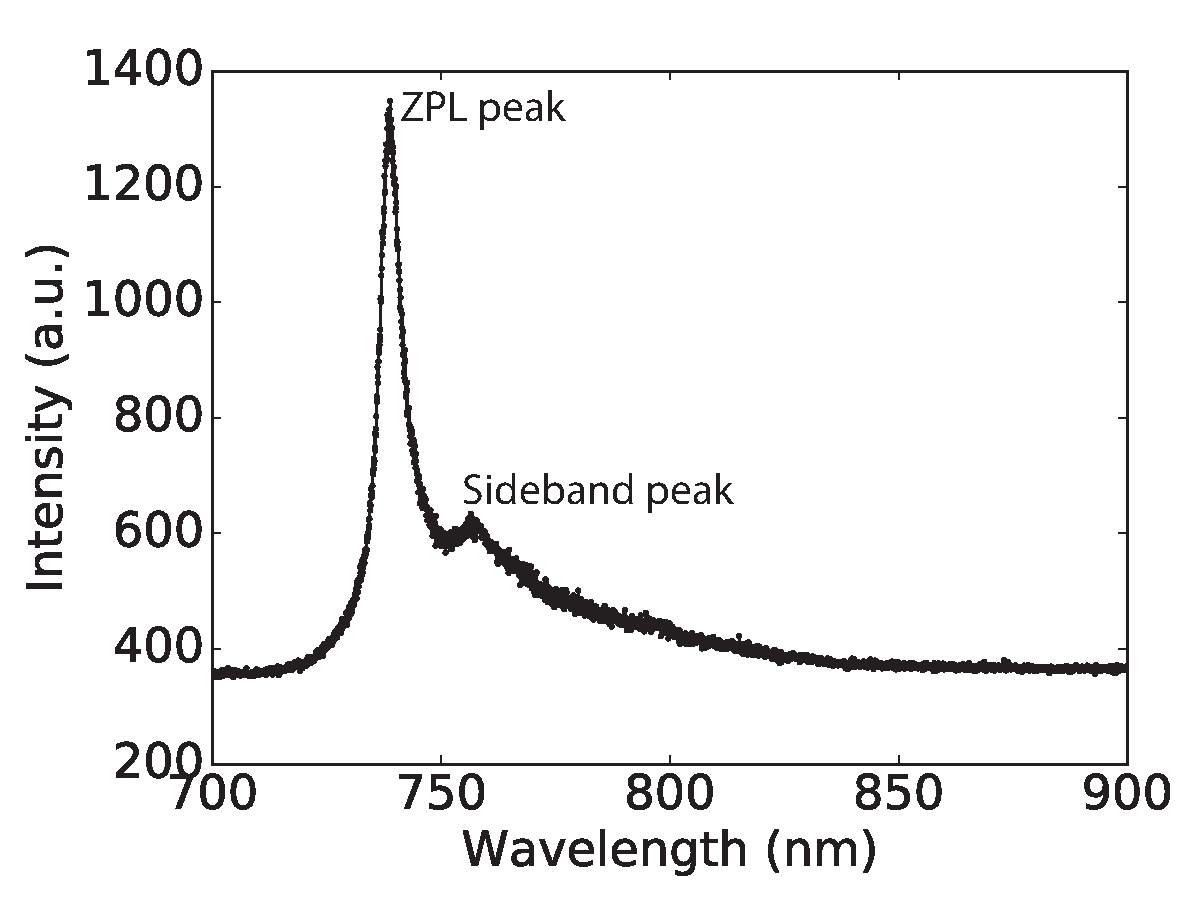
\includegraphics[trim = 0 0 0 0,  clip = true, width = 0.49\textwidth]{./pics/Ir25M_spe_scan_xy-38x9y16_300uW_t120.pdf}}
			\caption{Representative spectrum of an emitter of \vl exhibiting a sideband peak.}
			\label{fig::broad_peak_sb}
		\end{figure}

		From literature it is known, that the \siv in \nd exhibits a large \db of over 70\% \cite{Neu2011,Neu2011b}, which is consistent with our measurements of \emnarrow and \embroad.
		Nevertheless, sideband peaks are present in many \siv PL emission spectra.
		The investigated emitters exhibit two different structures of sideband spectra: The spectra in \vl exhibit one strong sideband peak (\autoref{fig::broad_peak_sb}), spectra in \hl exhibit several weaker sideband peaks.
		\\
		However, there is no recurring pattern in the sideband of \hl.
		The challenge arises to unequivocally distinguish between peaks stemming from a phonon sideband and peaks stemming from shifted, less intense \siv \ZPLs.
		The possibility exists, that some peaks identified as phonon sidebands are actually ZPLs stemming from shifted \sivs. 
		Therefore, we will focus our investigations on the more prominent sideband of \vl.
		\\
		Most of the spectra in \vl exhibit a characteristic shape, composed of the ZPL and one strong sideband peak which is mostly shifted \SIrange{37}{43}{meV}. 
		In reference \cite{Dietrich2014} the \SI{42}{meV} sideband peak is attributed to a non-localized (lattice) mode. 
		It is also stated, that the local vibrational mode at \SI{64}{meV} is much stronger than the  \SI{42}{meV} sideband peak. 
		While the peak attributed to the non-localized mode is very strong in our measurements, we cannot identify the peak attributed to the local vibrational \siv mode in the spectra of \vl. 
		A possible explanation is, that the lattice mode at \SIrange{37}{43}{meV} is so strong that the local vibrational mode at \SI{64}{meV} cannot be separated from the tail of the lattice mode.
		In \autoref{fig::sideband_fit} the distance between the \cwl of the sideband peak and the \cwl of the ZPL is plotted against the ZPL \cwl. 
		The distribution is fitted with a linear regression.
		We attribute the variance in the sideband shift to strain: \correct{Adam Galis Erkenntnisse}
		\\
		